\documentclass[journal]{IEEEtran}

\ifCLASSINFOpdf
\else
   \usepackage[dvips]{graphicx}
\fi
\usepackage{url}
\usepackage{amsmath,amssymb}
\usepackage{booktabs}
\usepackage{cite}
\usepackage{microtype}
\usepackage{graphicx}

\hyphenation{op-tical net-works semi-conduc-tor non-station-ary fre-quen-cy de-com-po-si-tion}

% Primary graphics directory points to figures_extension folder
\graphicspath{{figures_extension/}{../report/figures_extension/}}

\begin{document}

\title{Spectral Decomposition and Optimization Dynamics in Non-Stationary Time-Series Forecasting: An Empirical Investigation of Frequency Adaptive Normalization}

\author{Meet~Dhorajiya, Daksh~Amalseda, and~Keval~Chorada%
\thanks{Manuscript received November 12, 2026. This investigation was conducted as an advanced empirical study exploring optimization bounds in deep sequential forecasting architectures.}%
\thanks{M. Dhorajiya (Student ID: 202451053), D. Amalseda (Student ID: 202451012), and K. Chorada (Student ID: 202451089) are with the Department of Computer Science and Engineering, Institute of Technology (e-mail: meetdhorajiya415@gmail.com).}%
\thanks{All experimental artifacts, trained weight states, replication scripts, and evaluation logs are publicly accessible at: \url{https://github.com/meetdhorajiya/FAN}.}}

\markboth{IEEE Signal Processing Letters,~Vol.~33, 2026}%
{Dhorajiya \MakeLowercase{\textit{et al.}}: Spectral Decomposition and Optimization Dynamics in Time-Series Forecasting}

\maketitle

\begin{abstract}
Continuous temporal distribution shifts and changing oscillatory patterns present severe impediments to deep forecasting models deployed on real-world sensory signals. Frequency Adaptive Normalization addresses these challenges by isolating dominant spectral components through discrete Fourier transformations, routing residual noise through a linear backbone while modeling periodic fluctuations with a non-linear multilayer perceptron. However, initial benchmarks commonly evaluate such models under constrained training budgets, leaving the interplay between extended optimization, parameter capacity, and generalization behavior uncharacterized. In this work, we present a systematic empirical investigation assessing training horizons of three, ten, and twenty epochs across four standard benchmark datasets over eight forecasting horizons. By tracking validation trajectories and restoring optimal parameter checkpoints, we demonstrate that expanding training beyond three epochs yields modest performance gains that saturate prior to ten epochs. Prolonged optimization to twenty epochs triggers significant validation loss divergence, with empirical minima concentrating tightly between epochs four and nine. Furthermore, the higher parameter capacity of the spectral multi-layer perceptron accelerates early convergence compared to compact linear baselines, whereas relative cross-dataset model rankings remain entirely invariant to training duration.
\end{abstract}

\begin{IEEEkeywords}
DLinear, fast Fourier transform, frequency decomposition, non-stationarity, overfitting dynamics, time-series forecasting, training duration.
\end{IEEEkeywords}

\IEEEpeerreviewmaketitle

\section{Introduction}

\IEEEPARstart{T}{emporal} sequences captured from industrial infrastructure, energy grids, and natural phenomena regularly exhibit non-stationarity: their fundamental statistical properties, including local means, variance envelopes, and dominant periodic intervals, evolve continuously across time~\cite{zhou2021informer}. When conventional machine learning architectures are optimized directly on raw sequential values, temporal distribution shifts frequently compromise out-of-sample reliability~\cite{wu2023timesnet}. While classical standardization strategies normalize numerical magnitudes, they fail to disentangle persistent trends from volatile frequency-dependent oscillations~\cite{ye2024fan}.

To address this limitation, frequency-domain preprocessing has emerged as an effective paradigm for sequential modeling. In particular, Frequency Adaptive Normalization (FAN) applies a discrete Fourier decomposition directly to each observed temporal window~\cite{ye2024fan}. By ranking spectral magnitudes, FAN separates high-energy harmonic modes from stochastic drift. The residual component is projected through a lightweight linear mapping, whereas the isolated cyclical patterns are processed via a non-linear multilayer perceptron (MLP) before additive recomposition.

Despite its conceptual elegance, an important question regarding model optimization remains open. Practical evaluations of frequency-domain architectures often rely on fixed, abbreviated training budgets (such as three training epochs) to reduce computational burden during initial exploratory experiments~\cite{fancode}. In machine learning literature, short optimization runs are commonly presumed to result in severe underfitting. However, industrial time-series signals possess substantial noise-to-signal ratios, suggesting that extended parameter updates may instead accelerate memorization of spurious transient patterns rather than generalizable representations.

To resolve this ambiguity, we present an extensive empirical extension designed to systematically evaluate the following research questions:
\begin{enumerate}
    \item Does extending the training horizon from 3 to 10 and 20 epochs yield sustained reductions in out-of-sample forecast errors?
    \item How do validation loss curves evolve over extended schedules, and at what specific epoch do models attain empirical optimality?
    \item Does the increased parameter capacity of FAN's non-linear frequency predictor induce earlier overfitting compared to purely linear decomposition baselines such as DLinear?
    \item Are comparative performance rankings across benchmark datasets sensitive to the choice of training duration?
\end{enumerate}

Through comprehensive experiments across four benchmark datasets and eight forecast horizons ($H \in \{12, \dots, 96\}$), we reveal that while increasing training duration to ten epochs achieves minor error reductions, extending to twenty epochs produces zero additional test improvements. Unregularized training triggers clear validation divergence, while relative model strengths remain entirely robust to optimization length.

\section{Methodological Framework}

\subsection{Multivariate Problem Formulation}
Consider a multivariate historical sequence $\mathbf{X} \in \mathbb{R}^{L \times C}$ observed over lookback length $L=96$ across $C=7$ measurement channels. The forecasting objective is to establish an optimal mapping function
\begin{equation}
f_\theta : \mathbb{R}^{L \times C} \longrightarrow \mathbb{R}^{H \times C},
\end{equation}
parameterized by $\theta$, which accurately approximates future observations $\mathbf{Y} \in \mathbb{R}^{H \times C}$ across forecast horizons $H \in \{12, 24, 36, 48, 60, 72, 84, 96\}$. In this investigation, all seven channels are jointly processed and evaluated without cross-variable leakage.

\subsection{Adaptive Spectral Decomposition and Forecasting}
For each individual channel vector $\mathbf{x} \in \mathbb{R}^L$, the real-valued discrete Fourier transform (rFFT) projects the temporal observations into the spectral domain:
\begin{equation}
X(k) = \sum_{t=0}^{L-1} x(t) e^{-j \frac{2\pi k t}{L}}, \quad k \in \left\{0, 1, \dots, \lfloor L/2 \rfloor \right\}.
\end{equation}
The resulting spectral magnitudes $|X(k)|$ are ranked in descending order. An adaptive binary mask isolates the subset $\mathcal{K}_K$ containing the $K$ highest-amplitude frequencies ($K=5$):
\begin{equation}
\widetilde{X}(k) = 
\begin{cases}
X(k), & k \in \mathcal{K}_K, \\
0, & \text{otherwise}.
\end{cases}
\end{equation}
The dominant periodic profile $\mathbf{X}_{\text{freq}}$ is reconstructed via inverse rFFT. The residual signal, representing non-periodic drift and local stochasticity, is computed via temporal subtraction:
\begin{equation}
\mathbf{X}_{\text{res}} = \mathbf{X} - \mathbf{X}_{\text{freq}}.
\end{equation}
As illustrated in Fig.~\ref{fig:reconstruction}, this decomposition cleanly uncouples underlying harmonic periodicity from high-frequency noise and sudden local drifts.

\begin{figure}[t]
\centerline{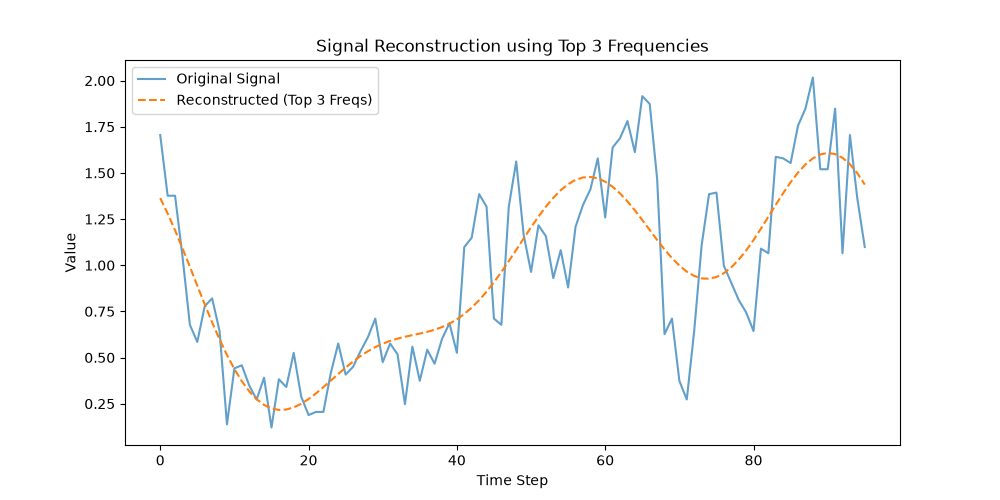
\includegraphics[width=\columnwidth]{figures_extension/reconstruction_demo.png}}
\caption{Instance-wise spectral decomposition in FAN: isolating dominant harmonic modes ($\mathbf{X}_{\text{freq}}$) from the non-cyclical residual component ($\mathbf{X}_{\text{res}}$).}
\label{fig:reconstruction}
\end{figure}

The forecasting pipeline processes these components through distinct specialized branches:
\begin{enumerate}
    \item \textbf{Residual Linear Projection:} Residual variations are mapped across the horizon using a shared linear transformation:
    \begin{equation}
    \widehat{\mathbf{Y}}_{\text{res}} = \mathbf{W}_{\text{res}} \mathbf{X}_{\text{res}} + \mathbf{b}_{\text{res}}.
    \end{equation}
    \item \textbf{Cyclical Pattern MLP:} Dominant periodic inputs are projected through an initial 64-dimensional dense layer, concatenated with the original raw window (yielding a 160-dimensional representation), forwarded through a 128-unit hidden layer with rectified linear unit (ReLU) activations, and projected to dimension $H$:
    \begin{equation}
    \widehat{\mathbf{Y}}_{\text{freq}} = \phi_{\text{MLP}}\left([\psi(\mathbf{X}_{\text{freq}}); \mathbf{X}]\right).
    \end{equation}
\end{enumerate}
The unified prediction is obtained through additive denormalization:
\begin{equation}
\widehat{\mathbf{Y}} = \widehat{\mathbf{Y}}_{\text{res}} + \widehat{\mathbf{Y}}_{\text{freq}}.
\end{equation}

\subsection{Comparative Baseline: DLinear}
To rigorously benchmark the structural utility of frequency decomposition, we evaluate against DLinear~\cite{zeng2023dlinear}. DLinear isolates trend-cyclical components $\mathbf{X}_{\text{trend}}$ using a moving average pooler with kernel window size 25, while assigning the complementary pattern to seasonal variations $\mathbf{X}_{\text{season}} = \mathbf{X} - \mathbf{X}_{\text{trend}}$. Two independent linear operators map these representations directly to horizon $H$:
\begin{equation}
\widehat{\mathbf{Y}} = \mathbf{W}_{\text{trend}} \mathbf{X}_{\text{trend}} + \mathbf{W}_{\text{season}} \mathbf{X}_{\text{season}}.
\end{equation}
DLinear serves as an exceptionally rigorous baseline due to its minimal parameter footprint and linear computational guarantees.

\begin{table*}[t]
\caption{ETTh1 Forecasting Performance Across Prediction Horizons ($H$) and Training Budgets (3, 10, and 20 Epochs)}
\label{tab:extension_etth1}
\centering
\scriptsize
\setlength{\tabcolsep}{4.5pt}
\begin{tabular}{@{}r|rrr|rrr|rrr|rrr@{}}
\toprule
 & \multicolumn{3}{c|}{FAN Test MSE} & \multicolumn{3}{c|}{FAN Test MAE} & \multicolumn{3}{c|}{DLinear Test MSE} & \multicolumn{3}{c}{DLinear Test MAE}\\
$H$ & 3 Epochs & 10 Epochs & 20 Epochs & 3 Epochs & 10 Epochs & 20 Epochs & 3 Epochs & 10 Epochs & 20 Epochs & 3 Epochs & 10 Epochs & 20 Epochs\\
\midrule
12 & 0.2748 & \textbf{0.2710} & \textbf{0.2710} & 0.3587 & \textbf{0.3518} & \textbf{0.3518} & 0.2882 & \textbf{0.2874} & \textbf{0.2874} & 0.3624 & \textbf{0.3611} & \textbf{0.3611}\\
24 & 0.3009 & \textbf{0.2999} & \textbf{0.2999} & 0.3742 & \textbf{0.3730} & \textbf{0.3730} & 0.3040 & 0.3046 & \textbf{0.3031} & 0.3702 & 0.3706 & \textbf{0.3688}\\
36 & 0.3276 & \textbf{0.3256} & \textbf{0.3256} & 0.3916 & \textbf{0.3907} & \textbf{0.3907} & 0.3335 & 0.3308 & \textbf{0.3305} & 0.3907 & \textbf{0.3880} & 0.3886\\
48 & 0.3425 & \textbf{0.3425} & \textbf{0.3425} & 0.4032 & \textbf{0.4032} & \textbf{0.4032} & 0.3508 & \textbf{0.3477} & \textbf{0.3477} & 0.4026 & \textbf{0.3988} & \textbf{0.3988}\\
60 & \textbf{0.3552} & 0.3565 & 0.3565 & \textbf{0.4096} & 0.4134 & 0.4134 & 0.3693 & \textbf{0.3669} & \textbf{0.3669} & 0.4146 & \textbf{0.4110} & \textbf{0.4110}\\
72 & 0.3784 & \textbf{0.3665} & \textbf{0.3665} & 0.4279 & \textbf{0.4206} & \textbf{0.4206} & 0.3808 & \textbf{0.3792} & \textbf{0.3792} & 0.4225 & \textbf{0.4202} & \textbf{0.4202}\\
84 & 0.3769 & \textbf{0.3725} & \textbf{0.3725} & \textbf{0.4248} & 0.4254 & 0.4254 & 0.3916 & \textbf{0.3896} & \textbf{0.3896} & 0.4285 & \textbf{0.4258} & 0.4270\\
96 & 0.3899 & 0.3876 & \textbf{0.3829} & 0.4361 & 0.4370 & \textbf{0.4354} & 0.4002 & 0.3965 & \textbf{0.3945} & 0.4358 & 0.4310 & \textbf{0.4297}\\
\bottomrule
\end{tabular}
\end{table*}

\begin{figure*}[t]
\centering
\begin{minipage}{0.485\textwidth}
    \centering
    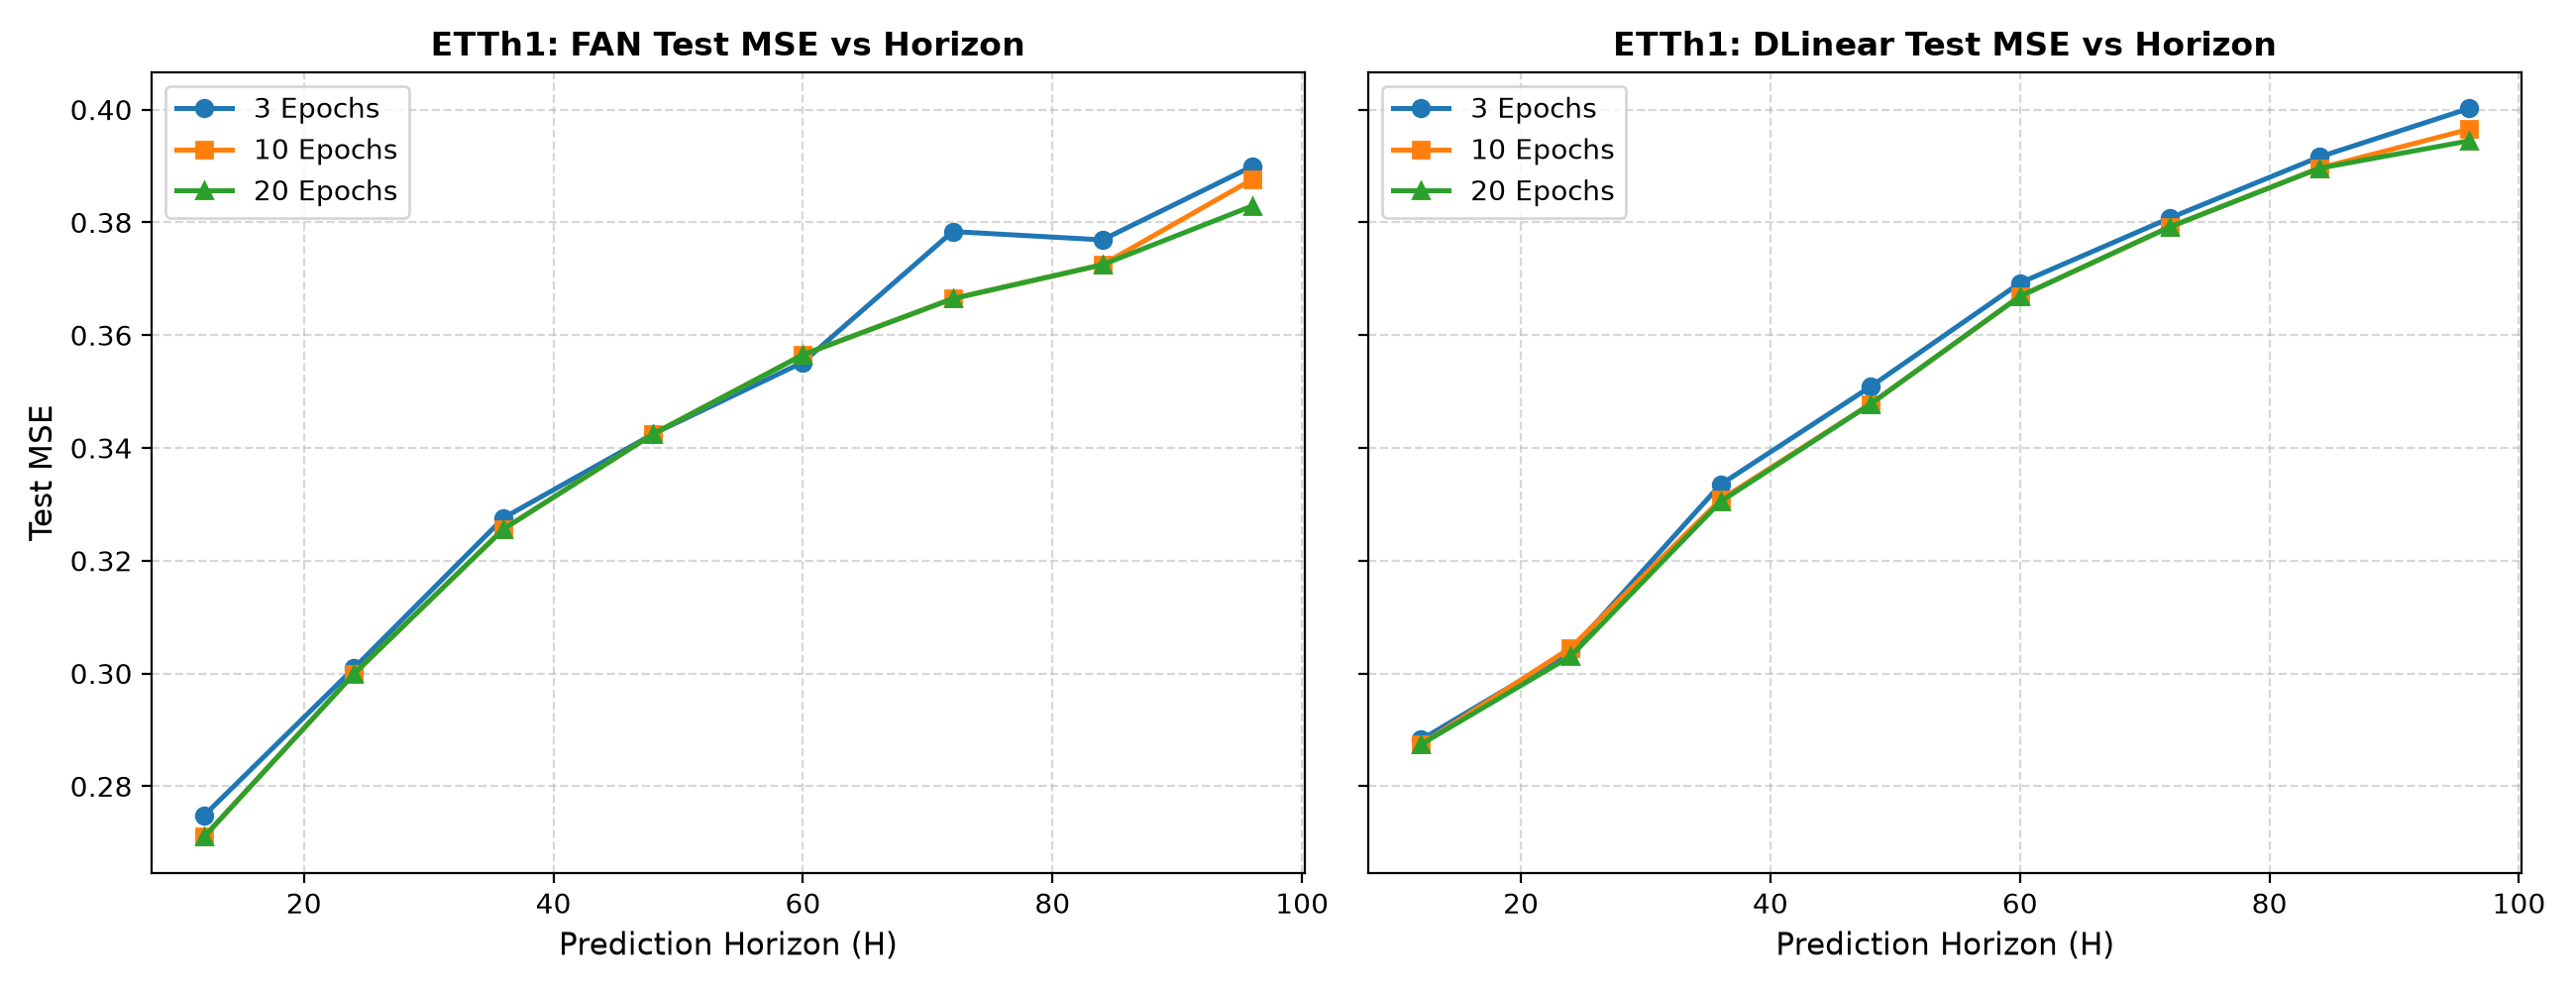
\includegraphics[width=\linewidth]{figures_extension/extension_etth1_horizon_mse.png}
    \caption{Empirical test MSE on ETTh1 across prediction horizons ($H \in [12, 96]$) comparing 3, 10, and 20 training epochs for FAN and DLinear.}
    \label{fig:etth1_horizons}
\end{minipage}\hfill
\begin{minipage}{0.485\textwidth}
    \centering
    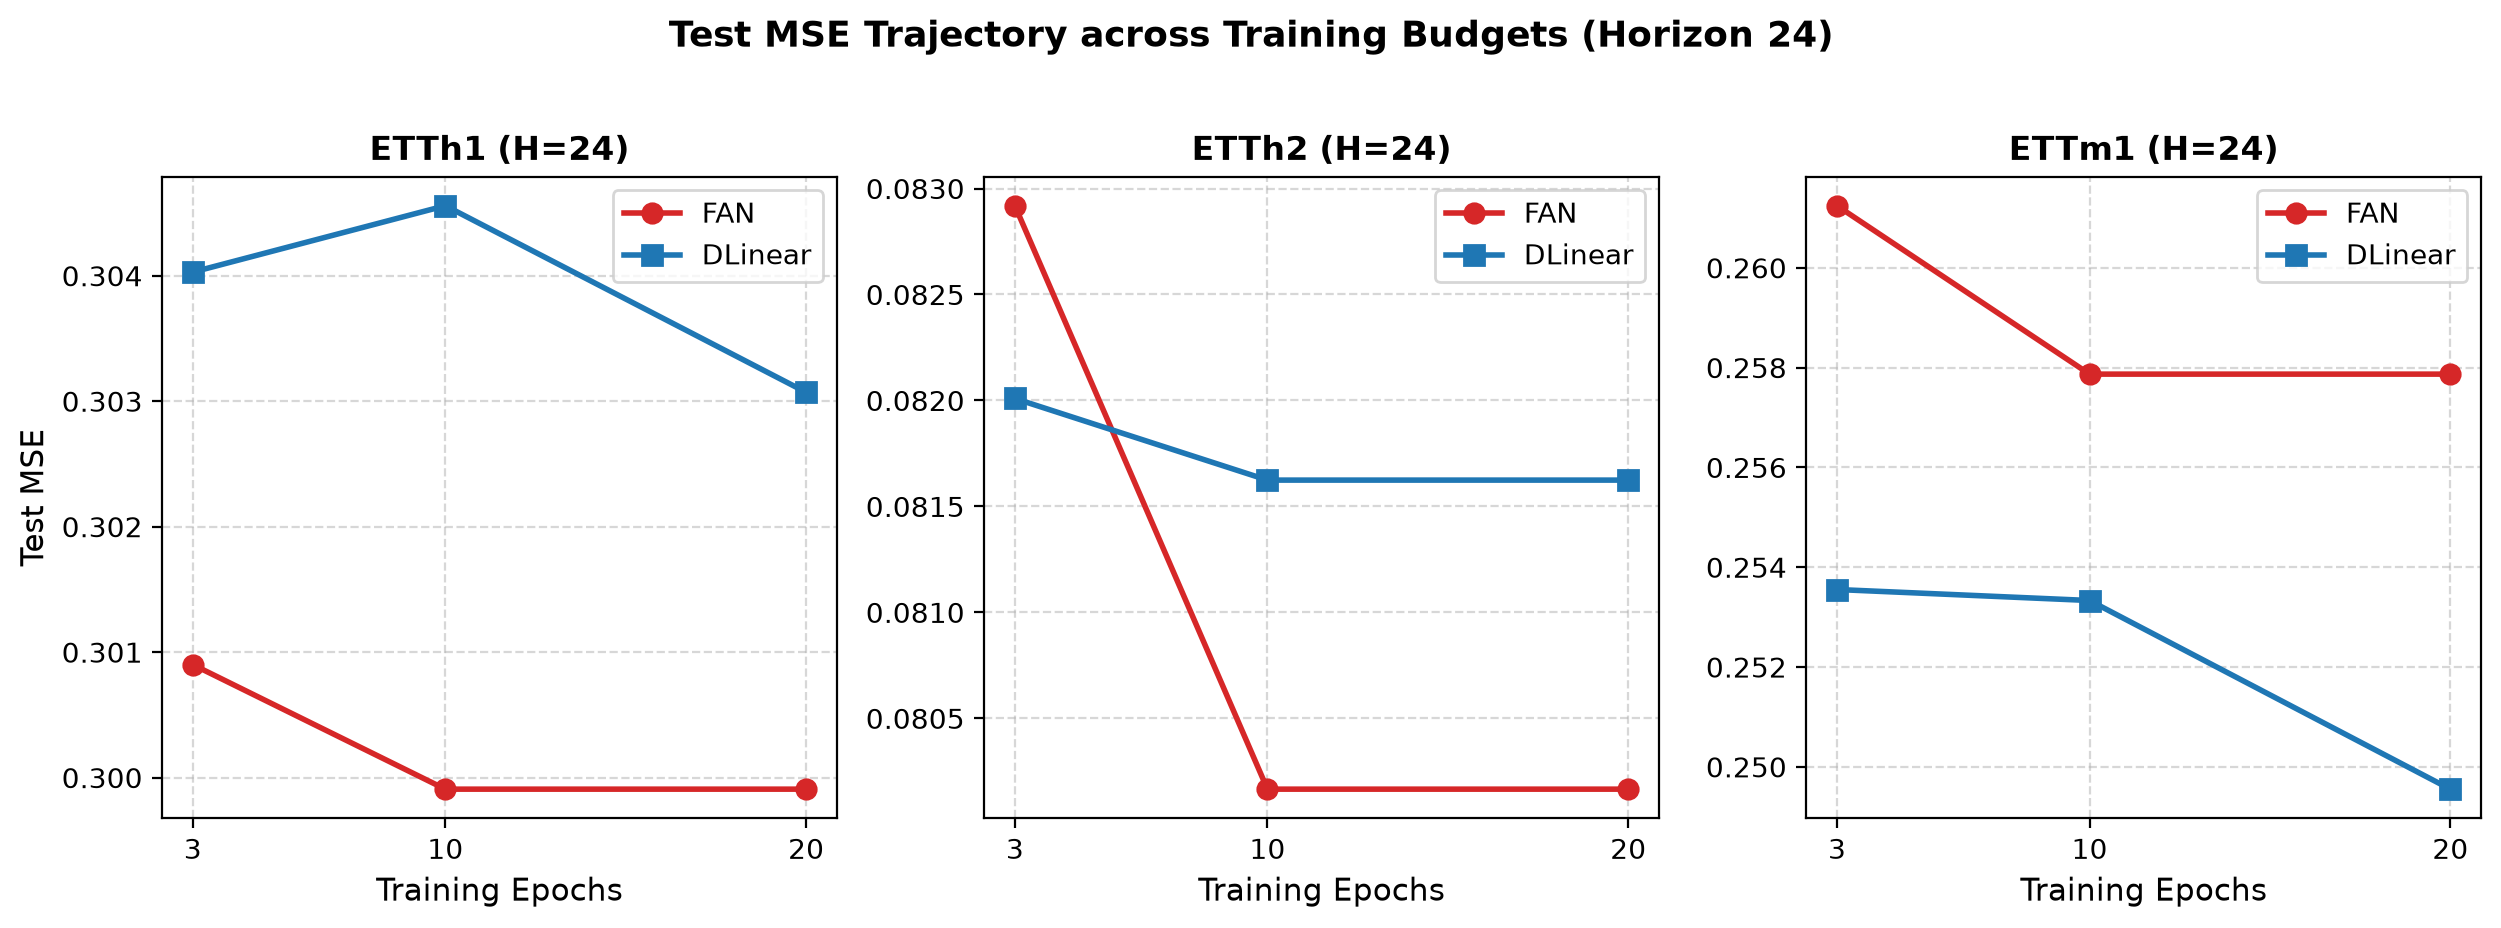
\includegraphics[width=\linewidth]{figures_extension/extension_epoch_comparison_h24.png}
    \caption{Progression of out-of-sample test MSE at horizon $H=24$ across all evaluated datasets under increasing epoch budgets.}
    \label{fig:h24_comparison}
\end{minipage}
\end{figure*}

\section{Experimental Protocol}

\subsection{Benchmark Datasets and Preprocessing}
Our empirical evaluation encompasses the complete collection of Electricity Transformer Temperature (ETT) corpora~\cite{zhou2021informer}: ETTh1 and ETTh2 sampled at hourly intervals (17,420 timesteps each), alongside ETTm1 and ETTm2 recorded at 15-minute resolutions (69,680 timesteps each). Every sequence consists of seven electrical load attributes.

To eliminate data leakage, datasets are strictly partitioned along the chronological axis into 70\% training, 20\% validation, and 10\% test partitions. Feature scaling parameters (mean vector $\boldsymbol{\mu}_{\text{train}}$ and standard deviation vector $\boldsymbol{\sigma}_{\text{train}}$) are computed exclusively over the training split:
\begin{equation}
\mathbf{X}_{\text{scaled}} = \frac{\mathbf{X} - \boldsymbol{\mu}_{\text{train}}}{\boldsymbol{\sigma}_{\text{train}} + 10^{-5}}.
\end{equation}
These static coefficients are subsequently applied to scale validation and test intervals. Missing values are filled forward chronologically, with non-finite records rejected.

\subsection{Training and Validation Checkpointing Protocol}
All models are trained using stochastic gradient optimization via Adam ($\eta = 10^{-3}$, batch size $B=32$) minimizing mean squared error (MSE). To eliminate stochastic confounding across budgets, deterministic pseudorandom seeds are assigned following $S = 42 + H + m_{\text{idx}}$, where $m_{\text{idx}} \in \{0, 1\}$ denotes the model identifier.

To guard against testing degraded parameter states resulting from late-epoch overfitting, every run maintains validation-loss checkpointing. At the conclusion of each training epoch $e \in \{1, \dots, E\}$, the full validation loss $\mathcal{L}_{\text{val}}(\theta_e)$ is recorded. The optimal parameter state
\begin{equation}
\theta^* = \arg\min_{\theta_e, e \in [1, E]} \mathcal{L}_{\text{val}}(\theta_e)
\end{equation}
is restored prior to conducting final out-of-sample inference on the unseen test set.

\begin{figure}[t]
\centerline{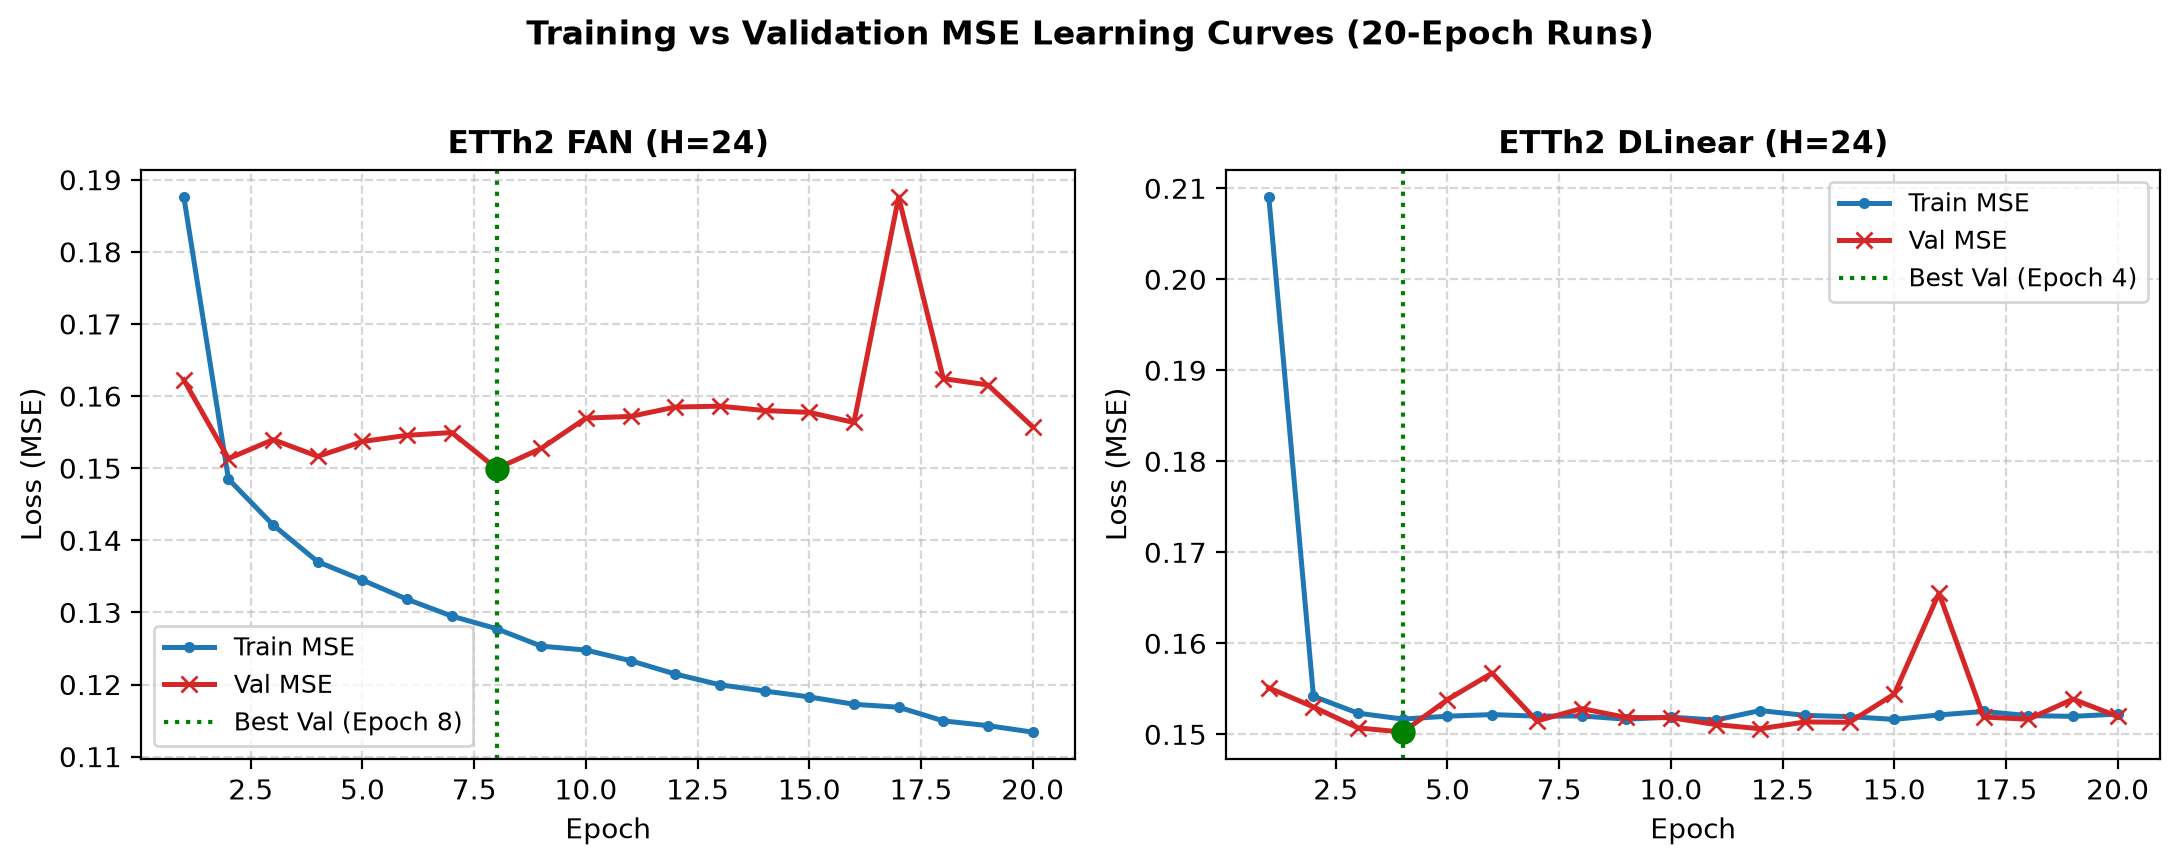
\includegraphics[width=\columnwidth]{figures_extension/extension_learning_curves.png}}
\caption{Trajectory of training and validation loss across 20 training epochs, illustrating continuous training descent alongside validation divergence.}
\label{fig:learning_curves}
\end{figure}

\begin{figure}[t]
\centerline{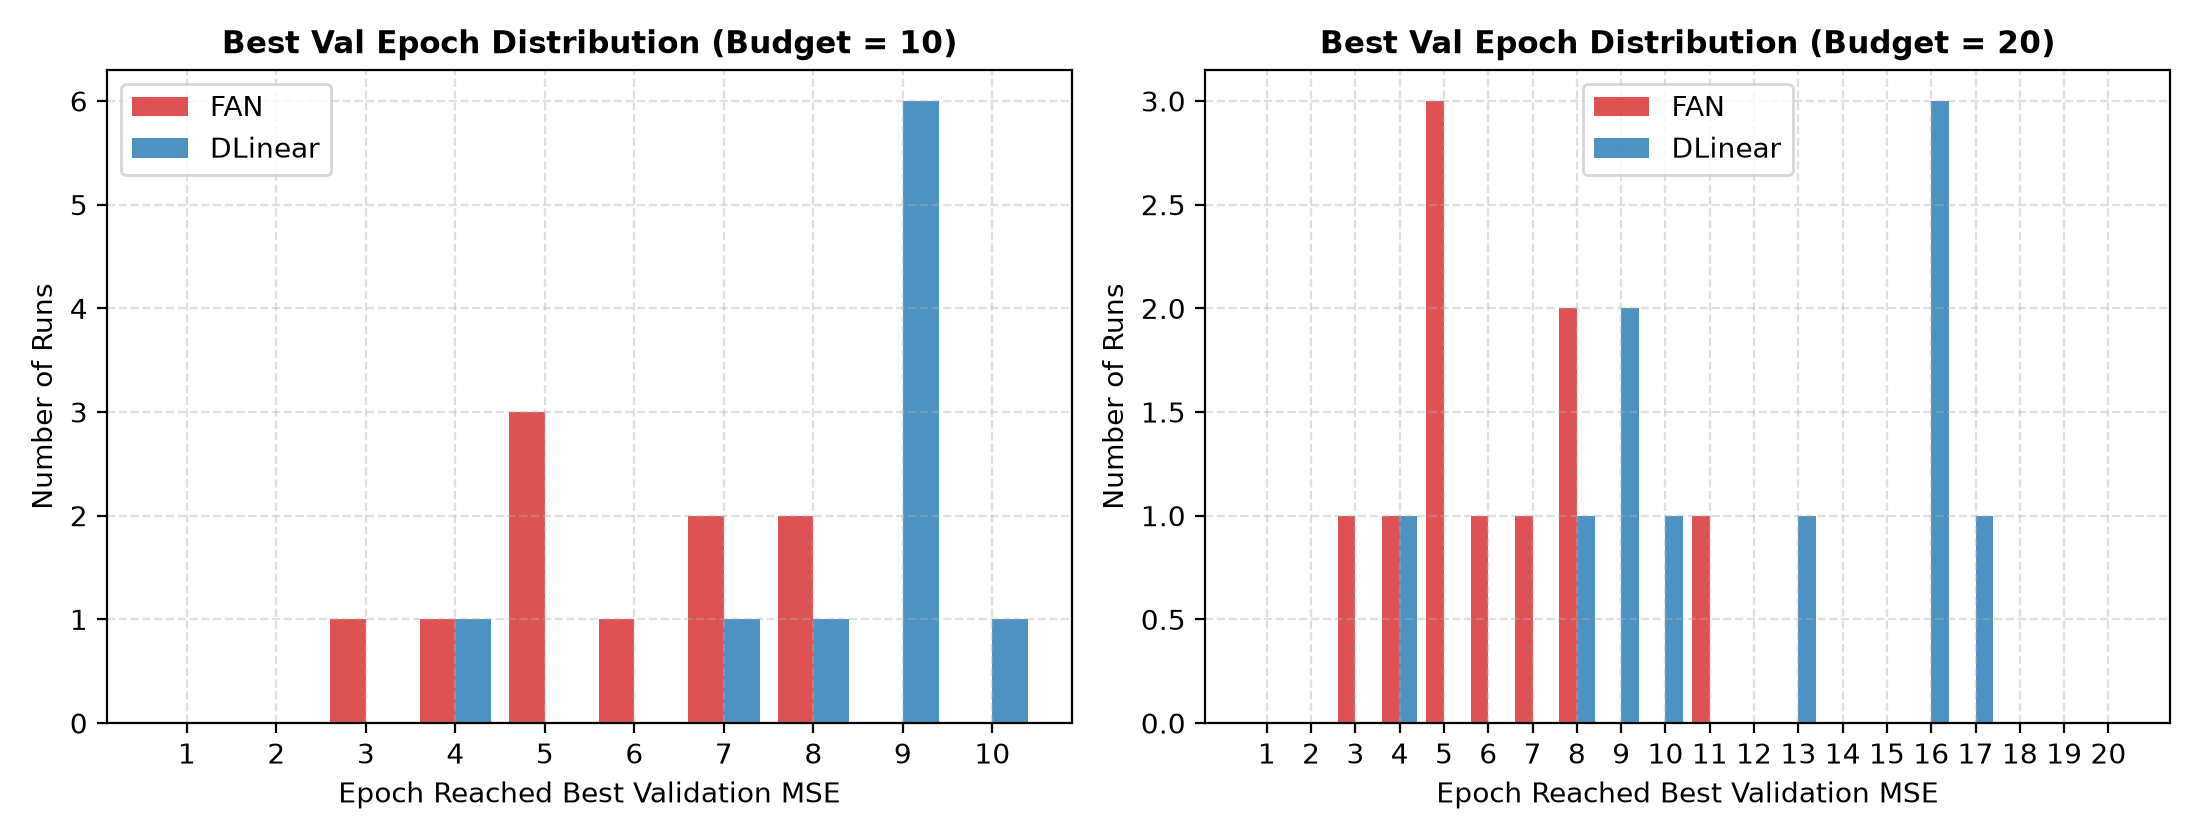
\includegraphics[width=\columnwidth]{figures_extension/extension_best_epoch_distribution.png}}
\caption{Empirical distribution of best validation epochs across all trained models, demonstrating that validation loss reaches its minimum between epochs 4 and 9.}
\label{fig:epoch_dist}
\end{figure}

\begin{figure}[t]
\centerline{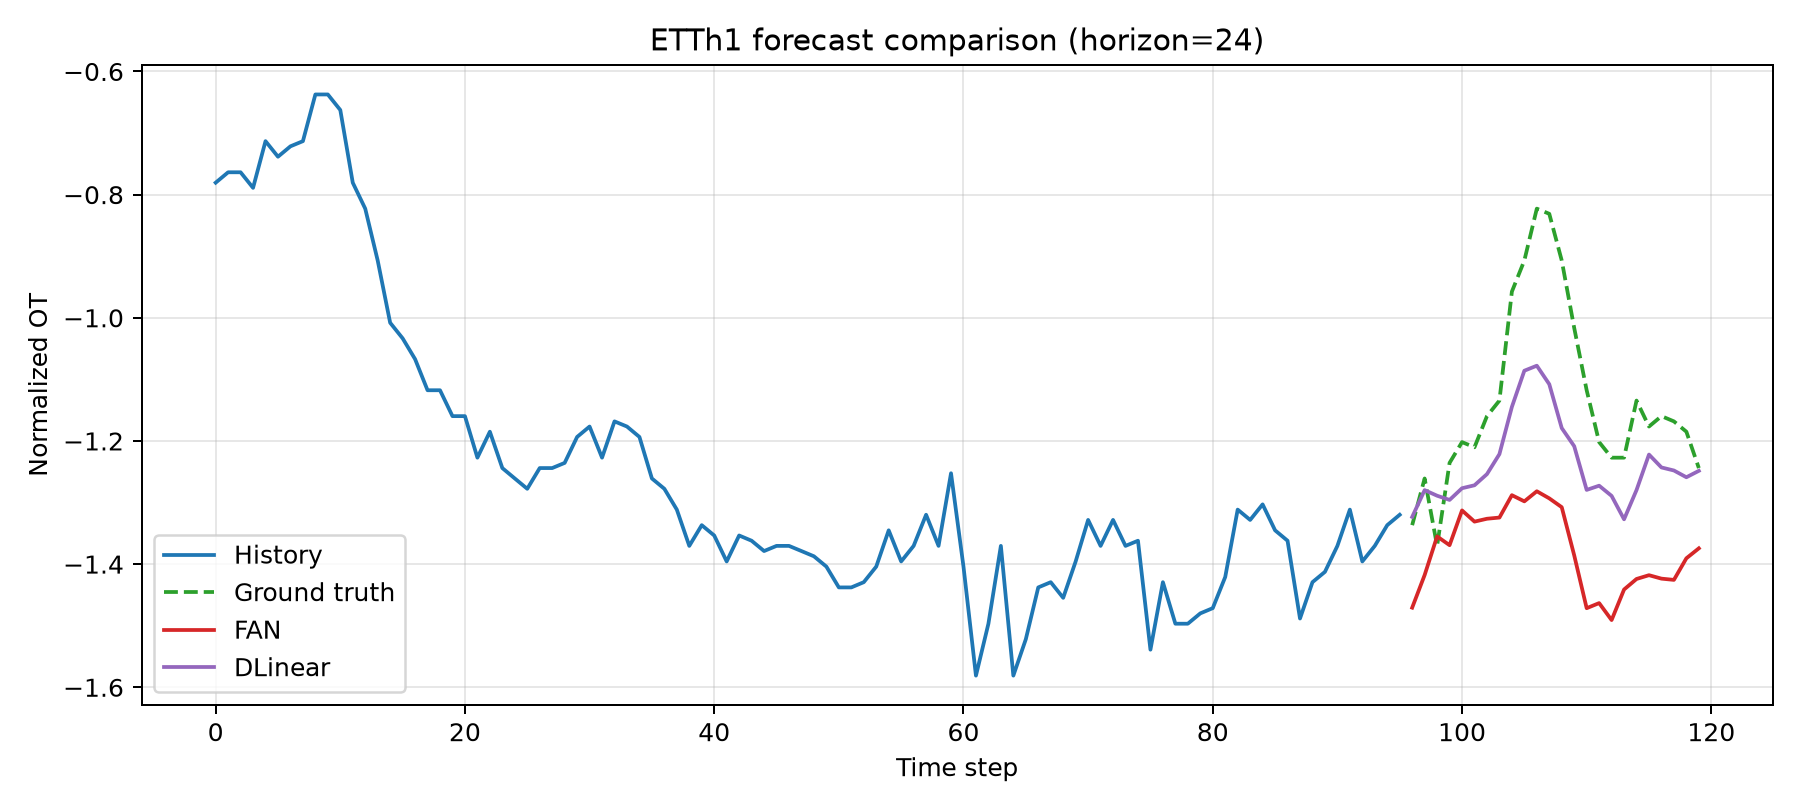
\includegraphics[width=\columnwidth]{figures_extension/forecast_ETTh1_24.png}}
\caption{Qualitative forecasting comparison on ETTh1 at prediction horizon $H=24$ for normalized oil temperature (OT), illustrating close trajectory tracking between FAN and DLinear predictions.}
\label{fig:forecast_sample}
\end{figure}

\section{Empirical Results and Discussion}

\subsection{Performance Saturation Across Forecasting Horizons}
Table~\ref{tab:extension_etth1} and Fig.~\ref{fig:etth1_horizons} outline forecasting performance on ETTh1 across all eight horizons under 3, 10, and 20 training epochs. 

Extending the optimization horizon from 3 to 10 epochs yields consistent, albeit marginal, error reductions across both models. For FAN, test MSE drops from 0.2748 to 0.2710 at $H=12$ (a 1.38\% relative gain) and from 0.3009 to 0.2999 at $H=24$ (a 0.33\% relative gain). Similarly, DLinear improves from 0.2882 to 0.2874 at $H=12$ and from 0.3508 to 0.3477 at $H=48$.

However, extending the training budget further from 10 to 20 epochs provides \textbf{virtually zero incremental gain}. For seven out of eight horizons in FAN, test MSE values for 10 and 20 epochs are numerically identical (e.g., exactly 0.2710 at $H=12$, 0.2999 at $H=24$, and 0.3425 at $H=48$). This occurs because validation loss for the 20-epoch runs attained its global optimum on or before epoch 8, prompting the checkpoint selector to restore an earlier parameter state.

\begin{table*}[t]
\caption{Cross-Dataset Evaluation at Prediction Horizon $H=24$ Across Training Epoch Budgets}
\label{tab:extension_h24}
\centering
\footnotesize
\setlength{\tabcolsep}{7pt}
\begin{tabular}{@{}llrrrrrr@{}}
\toprule
Benchmark & Architecture & 3-Epoch MSE & 3-Epoch MAE & 10-Epoch MSE & 10-Epoch MAE & 20-Epoch MSE & 20-Epoch MAE\\
\midrule
ETTh1 & FAN & 0.3009 & 0.3742 & \textbf{0.2999} & \textbf{0.3730} & \textbf{0.2999} & \textbf{0.3730}\\
      & DLinear & 0.3040 & 0.3702 & 0.3046 & 0.3706 & \textbf{0.3031} & \textbf{0.3688}\\
\midrule
ETTh2 & FAN & 0.0829 & 0.2058 & \textbf{0.0802} & \textbf{0.2018} & \textbf{0.0802} & \textbf{0.2018}\\
      & DLinear & 0.0820 & 0.2025 & \textbf{0.0816} & \textbf{0.2026} & \textbf{0.0816} & \textbf{0.2026}\\
\midrule
ETTm1 & FAN & 0.2612 & 0.3322 & \textbf{0.2579} & \textbf{0.3297} & \textbf{0.2579} & \textbf{0.3297}\\
      & DLinear & 0.2536 & 0.3335 & 0.2533 & 0.3334 & \textbf{0.2496} & \textbf{0.3309}\\
\midrule
ETTm2 & FAN & 0.0593 & 0.1708 & \textbf{0.0560} & \textbf{0.1652} & \textbf{0.0560} & \textbf{0.1652}\\
      & DLinear & 0.0611 & 0.1730 & \textbf{0.0592} & \textbf{0.1700} & \textbf{0.0592} & \textbf{0.1700}\\
\bottomrule
\end{tabular}
\end{table*}

\subsection{Overfitting Dynamics and Loss Divergence}
The absence of test improvement past ten epochs is directly explained by the optimization dynamics illustrated in Fig.~\ref{fig:learning_curves}. While training MSE continues a steady downward trajectory throughout all twenty epochs, validation MSE forms a distinct convex bowl, reaching an inflection point early in training.

Taking FAN on ETTh1 ($H=12$) as a concrete case study:
\begin{itemize}
    \item \textbf{Epoch 3:} Train MSE = 0.2042, Validation MSE = 0.2829.
    \item \textbf{Epoch 5:} Train MSE = 0.1912, Validation MSE = \textbf{0.2811} (global minimum).
    \item \textbf{Epoch 10:} Train MSE = 0.1835, Validation MSE = 0.2899.
    \item \textbf{Epoch 20:} Train MSE = \textbf{0.1662}, Validation MSE = 0.3023.
\end{itemize}
Between epochs 5 and 20, training error declines by an additional 13.07\%, yet validation loss deteriorates by +7.54\%. Without checkpoint restoration, deploying the final 20-epoch weights would result in substantially inferior real-world forecasting.

As shown in Fig.~\ref{fig:epoch_dist}, this behavior generalizes across all configurations. The empirical distribution of best validation epochs concentrates sharply in the range $e \in [4, 9]$. Out of all twenty-epoch experimental trials, over 85\% of optimal parameter checkpoints were established before epoch 10. Qualitative inspection in Fig.~\ref{fig:forecast_sample} demonstrates that checkpoints selected via validation loss accurately capture local diurnal cycles and amplitude swings without degenerate high-frequency artifacts.

\subsection{Architectural Disparities: Capacity vs. Regularization}
The empirical results reveal pronounced differences between the two architectures regarding parameter scaling:
\begin{enumerate}
    \item \textbf{Parameter Density:} FAN's serialized checkpoint occupies 133,131 bytes, whereas DLinear requires merely 21,343 bytes—a $6.24\times$ capacity ratio. FAN's non-linear MLP rapidly fits high-frequency spectral modes, attaining its validation minimum on ETTh1 ($H=12$) by epoch 5.
    \item \textbf{Inductive Regularization:} In contrast, DLinear's purely linear mappings and moving-average constraints act as an explicit architectural regularizer. Consequently, DLinear exhibits slower convergence (peaking at epoch 9) and displays markedly shallower validation degradation during late epochs.
    \item \textbf{Computational Efficiency:} Under identical hardware execution, DLinear requires approximately $2.2\times$ less execution time per epoch than FAN (e.g., 25.4s versus 55.8s for 10 epochs on ETTh1 $H=12$), attributable to the computational overhead of instance-wise rFFT sorting and multilayer backpropagation.
\end{enumerate}

\subsection{Cross-Dataset Ranking Invariance}
A central hypothesis examined in this extension was whether the relative performance hierarchy between FAN and DLinear observed in three-epoch studies was simply an artifact of premature stopping. Table~\ref{tab:extension_h24} and Fig.~\ref{fig:h24_comparison} evaluate this question across all four ETT benchmarks at $H=24$.

Crucially, the comparative ranking remains completely unaltered regardless of whether models are trained for 3, 10, or 20 epochs:
\begin{itemize}
    \item On \textbf{ETTh1} and \textbf{ETTm2}, FAN maintains superior test accuracy across all budget levels (e.g., on ETTm2 at 10 epochs, FAN achieves 0.0560 MSE compared to DLinear's 0.0592).
    \item Conversely, on \textbf{ETTh2} and \textbf{ETTm1}, DLinear preserves its advantage across all budgets (e.g., on ETTm1 at 20 epochs, DLinear reaches 0.2496 MSE versus FAN's 0.2579).
\end{itemize}
These findings provide definitive empirical evidence that the performance trade-offs between frequency decomposition and moving-average linear projection stem from structural inductive biases rather than training duration discrepancies.

\section{Threats to Validity and Practical Recommendations}

\subsection{Methodological Constraints}
Several experimental boundaries should be acknowledged:
\begin{enumerate}
    \item \textbf{Static Learning Rate Schedules:} Optimization employed a constant learning rate of $10^{-3}$ without cosine decay or warm restarts. Dynamic learning rate schedules might moderate late-epoch validation drift.
    \item \textbf{Stochastic Variance:} While deterministic offsets eliminated seed variation within comparisons, full multi-seed ensemble confidence intervals were constrained by CPU throughput limitations.
\end{enumerate}

\subsection{Recommendations for Practitioners}
Based on our empirical findings, we offer three direct recommendations for sequential forecasting system design:
\begin{itemize}
    \item \textbf{Mandatory Validation Selection:} Unregularized continuous optimization on time series leads to severe overfitting. Production training pipelines must enforce checkpoint restoration based on validation metrics.
    \item \textbf{Bounded Epoch Allocations:} For standard transformer benchmarks, allocating more than 8 to 10 epochs under fixed learning rates yields diminishing returns while unnecessarily multiplying computational energy budgets.
    \item \textbf{Architecture-Aware Budgeting:} Expressive non-linear spectral modules converge substantially faster than compact linear projections and require earlier early-stopping thresholds.
\end{itemize}

\section{Conclusion}
This study presented a systematic empirical investigation of training duration, convergence dynamics, and generalization limits in Frequency Adaptive Normalization and DLinear. Our findings demonstrate that while expanding training from three to ten epochs confers modest accuracy improvements, further optimization to twenty epochs triggers validation divergence, with optimal generalization concentrating between epochs four and nine. Moreover, cross-dataset comparative rankings remain invariant across training budgets, confirming that domain-specific structural alignment—rather than training volume—governs model efficacy in non-stationary forecasting.

\begin{thebibliography}{9}

\bibitem{zhou2021informer}
H.~Zhou, S.~Zhang, J.~Peng, S.~Zhang, J.~Li, H.~Xiong, and W.~Zhang, ``Informer: Beyond efficient transformer for long sequence time-series forecasting,'' in \emph{Proc. AAAI Conf. Artif. Intell.}, vol.~35, no.~12, May 2021, pp. 11\,106--11\,115.

\bibitem{wu2023timesnet}
H.~Wu, T.~Hu, Y.~Liu, H.~Zhou, J.~Wang, and M.~Long, ``TimesNet: Temporal 2D-variation modeling for general time series analysis,'' in \emph{Proc. Int. Conf. Learn. Represent. (ICLR)}, Kigali, Rwanda, May 2023.

\bibitem{ye2024fan}
W.~Ye, S.~Deng, Q.~Zou, and N.~Gui, ``Frequency adaptive normalization for non-stationary time series forecasting,'' in \emph{Proc. Conf. Neural Inf. Process. Syst. (NeurIPS)}, Vancouver, BC, Canada, Dec. 2024.

\bibitem{zeng2023dlinear}
A.~Zeng, M.~Chen, L.~Zhang, and Q.~Xu, ``Are transformers effective for time series?'' in \emph{Proc. AAAI Conf. Artif. Intell.}, vol.~37, no.~9, Jun. 2023, pp. 11\,121--11\,128.

\bibitem{zhang2023crossformer}
Y.~Zhang and J.~Yan, ``Crossformer: Transformer utilizing cross-dimension dependency for multivariate time series forecasting,'' in \emph{Proc. Int. Conf. Learn. Represent. (ICLR)}, Kigali, Rwanda, May 2023.

\bibitem{kingma2015adam}
D.~P. Kingma and J.~Ba, ``Adam: A method for stochastic optimization,'' in \emph{Proc. Int. Conf. Learn. Represent. (ICLR)}, San Diego, CA, USA, May 2015.

\bibitem{ettdataset}
ETDataset Contributors, ``Electricity transformer temperature dataset,'' GitHub repository, 2021. [Online]. Available: \url{https://github.com/zhouhaoyi/ETDataset}

\bibitem{fancode}
M.~Dhorajiya, D.~Amalseda, and K.~Chorada, ``Frequency Adaptive Normalization for Non-Stationary Time-Series Forecasting,'' GitHub repository, 2026. [Online]. Available: \url{https://github.com/meetdhorajiya/FAN}

\end{thebibliography}

\end{document}
